\chapter{Dynamique du cytosquelette et motilité cellulaire}\label{ch:b3:cytoskeleton-motility}

Un polynucléaire neutrophile qui poursuit une bactérie dans un tissu
rampe à dix micromètres par minute et change de direction en quelques
secondes quand l'odeur se déplace. Une vésicule de neurotransmetteur
fabriquée dans le corps cellulaire d'un motoneurone parcourt un mètre
le long de l'axone jusqu'au pied, tractée par une protéine motrice qui
fait des pas de huit nanomètres, cent par seconde, pendant quinze
jours. Les \omterm{def:b3:cytoskeleton-motility:cilia}{cils} qui tapissent la trachée battent douze fois par seconde
en ondes coordonnées qui remontent vers la gorge la poussière inhalée
d'une journée. Tout cela est l'œuvre de trois sortes de filaments
protéiques qui s'assemblent et se désassemblent en quelques secondes,
et de moteurs qui brûlent une molécule d'ATP par pas. Le cytosquelette
n'est pas un squelette au sens d'une charpente fixe~; c'est un jeu de
polymères en renouvellement constant, dont la dynamique \emph{est} le
mécanisme de la forme, de la division et du mouvement. Ce chapitre
traite des polymères et de leur cinétique, des moteurs et de la
physique qui les limite, de la reptation d'une cellule et du battement
des \omterm{def:b3:cytoskeleton-motility:cilia}{cils} et des flagelles.

\section{Trois polymères}

\begin{definition}[Filaments d'actine, microtubules, filaments intermédiaires]\label{def:b3:cytoskeleton-motility:filaments}
\index{filament d'actine}\index{microtubule}\index{filament intermédiaire}\index{polarité!des filaments}\index{centrosome}
Un \emph{filament d'actine} est un polymère hélicoïdal à deux brins
d'actine globulaire, épais de \qty{7}{nm}, chaque sous-unité occupant
\qty{2.7}{nm} le long de l'axe, et polaire~: l'extrémité \emph{barbée}
(plus) croît plus vite que l'extrémité \emph{pointue} (moins), et
chaque sous-unité porte un ATP hydrolysé après son incorporation. Un
\emph{microtubule} est un tube creux de \qty{25}{nm} de diamètre
extérieur, bâti de treize protofilaments de dimères de tubuline
$\alpha\beta$ (\qty{8}{nm} par dimère), polaire lui aussi, son
extrémité \emph{plus} croissant plus vite et son extrémité \emph{moins}
étant d'ordinaire ancrée au \emph{centrosome} près du noyau~; la
sous-unité $\beta$ hydrolyse son GTP après incorporation. Un
\emph{filament intermédiaire} est un câble de \qty{10}{nm} fait de
protéines en hélices superenroulées (kératines dans les épithéliums,
vimentine dans le mésenchyme, neurofilaments dans les axones, lamines
sous l'enveloppe nucléaire), apolaire, sans nucléotide, et bien plus
stable --- un câble qui porte la tension plutôt qu'une voie dynamique.
L'actine se tient surtout sous la membrane plasmique et dans les
protrusions~; les microtubules rayonnent depuis le centrosome et
servent de voies au transport à longue distance ainsi que de fuseau~;
les filaments intermédiaires donnent à la cellule et à son noyau leur
résistance mécanique.
\end{definition}

\begin{omfigure}
\begin{tikzpicture}[every node/.style={font=\scriptsize}, >=stealth]
  % actin
  \begin{scope}
    \foreach \i in {0,...,11} { \fill[omThm!70] ({\i*0.4},{0.12*sin(\i*60)}) circle (0.17); }
    \node[below, align=center] at (2.2,-0.5) {filament d'actine, \qty{7}{nm}\\hélice à deux brins, actine-ATP\\sous-unité \qty{2.7}{nm} le long de l'axe};
    \node[left] at (-0.3,0) {$-$ pointue}; \node[right] at (4.6,0) {barbée $+$};
  \end{scope}
  % microtubule
  \begin{scope}[xshift=7.2cm]
    \draw[thick, fill=omDef!25] (0,-0.55) rectangle (4.4,0.55);
    \foreach \y in {-0.35,-0.15,0.05,0.25} \draw[omDef] (0,\y) -- (4.4,\y);
    \foreach \x in {0.4,0.8,...,4.0} \draw[omDef] (\x,-0.55) -- (\x,0.55);
    \draw[thick] (4.4,0) ellipse (0.18 and 0.55); \draw[thick, fill=white] (4.4,0) ellipse (0.09 and 0.38);
    \node[below, align=center] at (2.2,-0.65) {microtubule, \qty{25}{nm}\\13 protofilaments de tubuline $\alpha\beta$ (GTP)\\dimère long de \qty{8}{nm}};
    \node[left] at (-0.2,0) {$-$}; \node[right] at (4.7,0) {$+$};
  \end{scope}
  % intermediate filament
  \begin{scope}[yshift=-2.9cm, xshift=3.6cm]
    \foreach \dd in {-0.12,0,0.12} \draw[omMeth!70!black, thick] plot[domain=0:4.4, samples=60] (\x, {\dd + 0.1*sin(\x*200 + \dd*400)});
    \node[below, align=center] at (2.2,-0.4) {filament intermédiaire, \qty{10}{nm}\\câble superenroulé (kératine, vimentine, lamine), sans polarité ni nucléotide};
  \end{scope}
\end{tikzpicture}

{\small Les trois filaments à l'échelle des diamètres. Les polymères
d'actine et de tubuline sont polaires et hydrolysent un nucléotide
après l'assemblage, ce qui les rend dynamiques~; le \omterm{def:b3:cytoskeleton-motility:filaments}{filament
intermédiaire} est un câble apolaire bâti pour l'endurance.}
\end{omfigure}

\begin{omfigure}
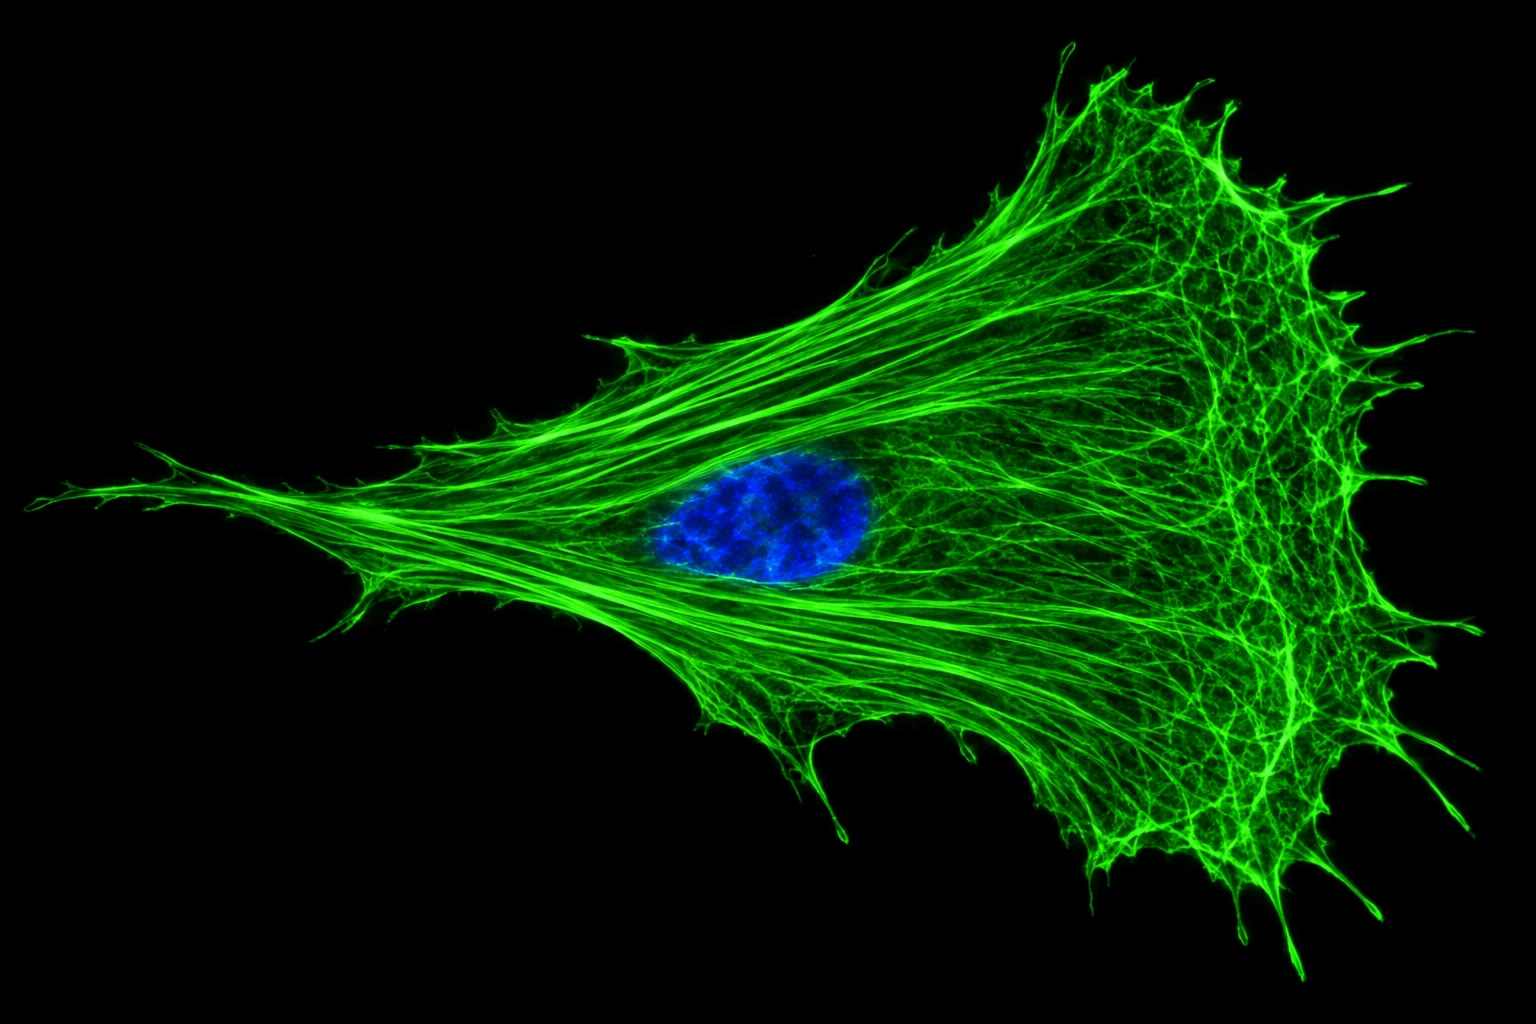
\includegraphics[width=0.54\linewidth]{images/book5/ai/b5-09-fibroblast-actin.jpg}\hspace{0.03\linewidth}
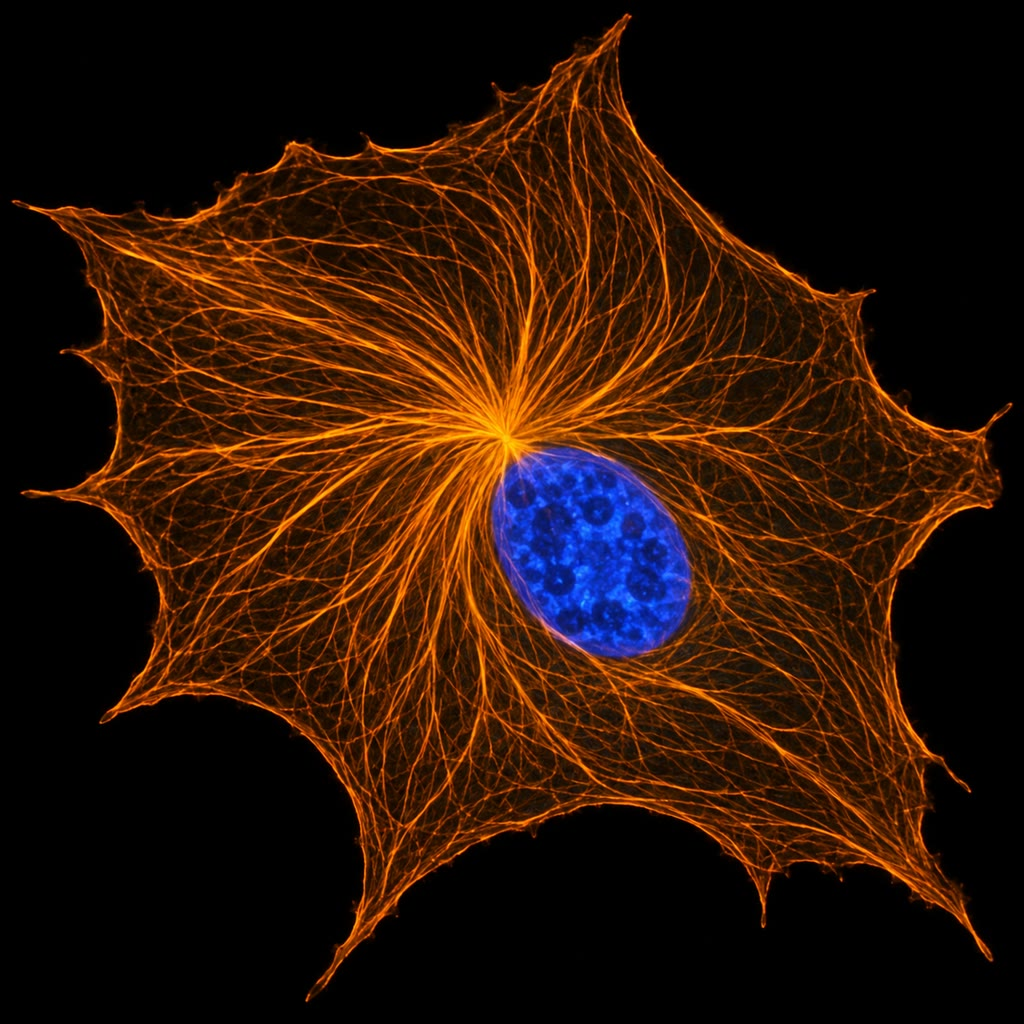
\includegraphics[width=0.36\linewidth]{images/book5/ai/b5-09-microtubules.jpg}

{\small À gauche~: l'actine (vert) dans un fibroblaste en migration ---
des fibres de tension en travers du corps, un réseau dense au large
bord avant, à droite. À droite~: les \omterm{def:b3:cytoskeleton-motility:filaments}{microtubules} (orange) rayonnant du
\omterm{def:b3:cytoskeleton-motility:filaments}{centrosome}, à côté du noyau (bleu), jusqu'à la marge cellulaire.}
\end{omfigure}

\section{La cinétique d'un polymère}

\begin{theorem}[Concentration critique et treadmilling]\label{thm:b3:cytoskeleton-motility:treadmilling}
\index{concentration critique}\index{treadmilling}
Soit une extrémité de filament qui ajoute des sous-unités à la vitesse
$k_{\text{on}}C$, $C$ étant la concentration de monomères libres, et en
perd à la vitesse $k_{\text{off}}$. Cette extrémité croît si $C$
dépasse sa \emph{\omterm{thm:b3:cytoskeleton-motility:treadmilling}{concentration critique}}
$C_{c} = k_{\text{off}}/k_{\text{on}}$ et décroît en deçà. Si les deux
extrémités ont des \omterm{thm:b3:cytoskeleton-motility:treadmilling}{concentrations critiques} différentes, $C_{c}^{+}
< C_{c}^{-}$, alors à l'état stationnaire où le filament ne s'allonge
ni ne se raccourcit la concentration de monomères vaut
\[
C_{\text{ss}} = \frac{k_{\text{off}}^{+} + k_{\text{off}}^{-}}
{k_{\text{on}}^{+} + k_{\text{on}}^{-}},
\qquad C_{c}^{+} < C_{\text{ss}} < C_{c}^{-},
\]
et l'extrémité plus croît tandis que l'extrémité moins décroît à la
même vitesse
$J = k_{\text{on}}^{+}C_{\text{ss}} - k_{\text{off}}^{+} > 0$~: les
sous-unités traversent le filament du plus vers le moins --- c'est le
\emph{treadmilling} --- au prix d'un nucléotide hydrolysé par
sous-unité.
\end{theorem}
\begin{proof}
La vitesse nette à une extrémité vaut
$k_{\text{on}}C - k_{\text{off}}$, nulle en $C_{c}$. Une longueur
constante exige que la somme des deux vitesses nettes s'annule, ce qui
donne $C_{\text{ss}}$~; celle-ci se trouve entre les deux
\omterm{thm:b3:cytoskeleton-motility:treadmilling}{concentrations critiques} parce qu'elle en est une moyenne pondérée
($C_{\text{ss}} =
(k_{\text{on}}^{+}C_{c}^{+} + k_{\text{on}}^{-}C_{c}^{-})/(k_{\text{on}}^{+}
+ k_{\text{on}}^{-})$). Au-dessus de $C_{c}^{+}$ l'extrémité plus
croît~; en deçà de $C_{c}^{-}$ l'extrémité moins décroît~; le flux est
la vitesse nette de l'extrémité plus. Deux extrémités d'un même
polymère chimique auraient le même $C_{c}$ (la même constante
d'équilibre), de sorte qu'une différence exige que la sous-unité change
après son incorporation --- l'hydrolyse de l'ATP ou du GTP --- ce qui
rend les extrémités dissemblables et paie le flux.
\end{proof}

\begin{example}[L'actine dans le tube à essai]\label{ex:b3:cytoskeleton-motility:actin-numbers}
Pour l'actine-ATP, $k_{\text{on}}^{+} = \qty{11.6}{\micro M^{-1}.s^{-1}}$,
$k_{\text{off}}^{+} = \qty{1.4}{s^{-1}}$ ($C_{c}^{+} = \qty{0.12}{\micro
M}$)~; $k_{\text{on}}^{-} = \qty{1.3}{\micro M^{-1}.s^{-1}}$,
$k_{\text{off}}^{-} = \qty{0.8}{s^{-1}}$ ($C_{c}^{-} = \qty{0.6}{\micro
M}$). Alors $C_{\text{ss}} = 2.2/12.9 = \qty{0.17}{\micro M}$ et $J =
11.6\times 0.17 - 1.4 = 0.6$ sous-unité par seconde~: \qty{1.6}{nm/s},
imperceptible. Dans une cellule les filaments font du treadmilling cent
fois plus vite, parce que la cofiline sectionne et dépouille de son
actine-ADP vieillie les extrémités pointues, la profiline charge de
l'actine-ATP fraîche sur les extrémités barbées, et des protéines de
coiffe décident quelles extrémités barbées ont le droit de croître~: le
polymère nu fournit le mécanisme, les régulateurs fournissent la
vitesse.
\end{example}

\begin{omfigure}
\begin{tikzpicture}
\begin{axis}[
  width=0.7\linewidth, height=5.6cm,
  axis x line=bottom, axis y line=left,
  xmin=0, xmax=1.0, ymin=-1.6, ymax=4,
  xlabel={actine libre ($\unit{\micro M}$)}, ylabel={vitesse nette (sous-unités/s)},
  xlabel style={font=\small, at={(axis description cs:0.5,-0.12)}, anchor=north},
  ylabel style={font=\small},
  tick label style={font=\small}, xtick={0,0.2,0.4,0.6,0.8,1.0}, ytick={-1,0,1,2,3,4},
  clip=false,
]
\addplot[thin, gray, domain=0:1.0, samples=2] {0};
\addplot[very thick, omThm, domain=0:0.46, samples=2] {11.6*x-1.4};
\addplot[very thick, omDef, domain=0:1.0, samples=2] {1.3*x-0.8};
\draw[dashed, gray] (axis cs:0.17,-1.6) -- (axis cs:0.17,4);
\node[font=\scriptsize, omThm, anchor=south east] at (axis cs:0.44,3.1) {extrémité barbée};
\node[font=\scriptsize, omDef, anchor=north west] at (axis cs:0.62,-0.25) {extrémité pointue};
\node[font=\scriptsize, anchor=south west] at (axis cs:0.19,3.5) {$C_{\text{ss}}$};
\fill[omThm] (axis cs:0.12,0) circle (2pt); \node[font=\scriptsize, anchor=north east] at (axis cs:0.11,-0.05) {$C_{c}^{+}$};
\fill[omDef] (axis cs:0.6,0) circle (2pt); \node[font=\scriptsize, anchor=south west] at (axis cs:0.61,0.05) {$C_{c}^{-}$};
\end{axis}
\end{tikzpicture}

{\small Vitesse nette de croissance de chaque extrémité d'un \omterm{def:b3:cytoskeleton-motility:filaments}{filament
d'actine} en fonction du monomère libre, avec les constantes de
l'exemple. Entre les deux \omterm{thm:b3:cytoskeleton-motility:treadmilling}{concentrations critiques}, l'extrémité barbée
croît et l'extrémité pointue décroît~; à la ligne pointillée les deux
se compensent exactement et le filament fait du treadmilling.}
\end{omfigure}

\begin{definition}[L'instabilité dynamique]\label{def:b3:cytoskeleton-motility:instability}
\index{instabilité dynamique}\index{coiffe GTP}\index{catastrophe}
Les \omterm{def:b3:cytoskeleton-motility:filaments}{microtubules} font plus étrange que du treadmilling. Une extrémité
plus en croissance porte une \emph{coiffe GTP} de dimères fraîchement
ajoutés~; derrière elle le GTP est hydrolysé, et la tubuline-GDP, qui
préfère une conformation courbe, est maintenue droite dans le réseau,
sous contrainte. Si la coiffe est perdue --- l'extrémité marque une
pause, ou la croissance ralentit --- les protofilaments contraints se
recourbent vers l'extérieur et le \omterm{def:b3:cytoskeleton-motility:filaments}{microtubule} raccourcit à
\qty{300}{nm/s}, vingt fois sa vitesse de croissance~: c'est une
\emph{catastrophe}, qui prend fin quand un dimère GTP se pose et
qu'une nouvelle coiffe se forme (un \emph{sauvetage}). Dans une même
population, certains \omterm{def:b3:cytoskeleton-motility:filaments}{microtubules} croissent donc pendant que leurs
voisins s'effondrent~: c'est l'\emph{instabilité dynamique}. Elle
permet à une cellule d'explorer son propre volume avec des extrémités
plus en quelques minutes et de rebâtir tout le réseau quand le
\omterm{def:b3:cytoskeleton-motility:filaments}{centrosome} se déplace ou que la cellule se divise. La cellule la règle
par des protéines qui suivent les extrémités plus, stabilisent (tau,
MAP2), sectionnent (katanine) ou dépolymérisent (kinésine-13) les
\omterm{def:b3:cytoskeleton-motility:filaments}{microtubules}~; la colchicine et les alcaloïdes de la pervenche bloquent
l'assemblage et le taxol le désassemblage, tous poisons du fuseau
mitotique employés contre le cancer.
\end{definition}

\begin{proof}[Faits expérimentaux]
Mitchison et Kirschner (1984) ont observé des populations de
\omterm{def:b3:cytoskeleton-motility:filaments}{microtubules} poussés à partir de \omterm{def:b3:cytoskeleton-motility:filaments}{centrosomes} in vitro. En diluant la
tubuline sous la \omterm{thm:b3:cytoskeleton-motility:treadmilling}{concentration critique}, ils s'attendaient à voir tous
les \omterm{def:b3:cytoskeleton-motility:filaments}{microtubules} raccourcir lentement~; au lieu de cela le nombre de
\omterm{def:b3:cytoskeleton-motility:filaments}{microtubules} chutait pendant que les survivants continuaient de
croître --- certains s'étaient désassemblés complètement et vite,
d'autres pas du tout. Des \omterm{def:b3:cytoskeleton-motility:filaments}{microtubules} isolés, filmés plus tard en
vidéomicroscopie, basculaient brusquement entre des phases de
croissance régulière et de raccourcissement rapide. La \omterm{def:b3:cytoskeleton-motility:instability}{coiffe GTP}
explique les deux~: seules les extrémités coiffées croissent, et la
perte de la coiffe est un événement rare, du tout ou rien.
\end{proof}

\section{Les moteurs}

\begin{definition}[Les protéines motrices]\label{def:b3:cytoskeleton-motility:motors}
\index{myosine}\index{kinésine}\index{dynéine}\index{processivité}
Une \emph{protéine motrice} convertit l'énergie libre de l'hydrolyse de
l'ATP en mouvement dirigé le long d'un filament~: les \emph{myosines}
le long de l'actine (la myosine~II, moteur du muscle et de la
contraction, vers l'extrémité barbée~; la myosine~V, porteuse de
vésicules à deux têtes qui fait des pas de \qty{36}{nm}), les
\emph{kinésines} le long des \omterm{def:b3:cytoskeleton-motility:filaments}{microtubules} vers l'extrémité plus (la
kinésine-1 fait des pas de \qty{8}{nm}, un dimère de tubuline, par ATP,
main sur main, à environ \qty{800}{nm/s}), et les \emph{dynéines} vers
l'extrémité moins (la dynéine cytoplasmique, avec son adaptateur la
dynactine, ramène la cargaison au centre de la cellule~; les \omterm{def:b3:cytoskeleton-motility:cilia}{dynéines
axonémales} courbent les \omterm{def:b3:cytoskeleton-motility:cilia}{cils}). Un moteur est \emph{processif} s'il fait
de nombreux pas avant de se détacher~: la kinésine-1 marche seule sur
environ un micromètre, une centaine de pas~; une tête isolée de
myosine~II ne fait qu'un coup de rame et lâche prise, de sorte qu'un
muscle a besoin de centaines de têtes travaillant sur un même filament.
Les moteurs lisent la polarité de la voie, de sorte que la géographie
d'une cellule --- extrémités plus à la périphérie, extrémités moins au
centre --- est la carte de l'endroit où chaque moteur portera sa
cargaison.
\end{definition}

\begin{proof}[Faits expérimentaux]
Vale, Reese et Sheetz (1985) ont identifié la \omterm{def:b3:cytoskeleton-motility:motors}{kinésine} comme la
protéine de l'axoplasme de calmar qui fait glisser des billes de latex
le long des \omterm{def:b3:cytoskeleton-motility:filaments}{microtubules} vers l'extrémité plus, et les années suivantes
ont démêlé la structure à deux têtes, la direction de chaque famille et
la partenaire rétrograde, la \omterm{def:b3:cytoskeleton-motility:motors}{dynéine}. Svoboda, Schmidt, Schnapp et
Block (1993) ont maintenu dans un piège optique une bille portant une
seule \omterm{def:b3:cytoskeleton-motility:motors}{kinésine} et ont enregistré sa position au nanomètre près~: la
bille avançait par pas discrets de \qty{8}{nm}, un par ATP à faible
concentration d'ATP, et calait contre une force d'environ \qty{6}{pN}.
L'escalier moléculaire avait été vu directement.
\end{proof}

\begin{omfigure}
\begin{tikzpicture}[every node/.style={font=\scriptsize}, >=stealth]
  % left: kinesin on a microtubule
  \begin{scope}
    \draw[thick, fill=omDef!25] (0,0) rectangle (5.4,0.5);
    \foreach \x in {0.4,0.8,...,5.2} \draw[omDef] (\x,0) -- (\x,0.5);
    \node[left] at (-0.1,0.25) {$-$}; \node[right] at (5.5,0.25) {$+$};
    % two heads, stalk, cargo
    \fill[omProp] (2.4,0.72) circle (0.2); \fill[omProp!60] (3.2,0.72) circle (0.2);
    \draw[thick, omProp!80!black] (2.6,0.85) -- (2.85,1.4) -- (3.05,0.85); \draw[thick, omProp!80!black] (2.85,1.4) -- (2.85,2.3);
    \draw[thick, fill=omExo!40] (2.85,2.7) circle (0.4); \node at (2.85,2.7) {cargaison};
    \draw[->, thick, omThm] (3.4,0.72) arc[start angle=180, end angle=0, radius=0.4] ; \node[right, omThm] at (3.85,1.15) {\qty{8}{nm} par ATP};
    \node[below, align=center] at (2.7,-0.1) {la kinésine-1 marche main sur main vers l'extrémité plus~;\\environ $100$ pas par seconde, \qty{0.8}{\micro m/s}};
  \end{scope}
  % right: optical trap staircase
  \begin{scope}[xshift=7.2cm, yshift=-0.6cm]
  \begin{axis}[
    width=5.6cm, height=4.4cm, axis lines=left,
    xmin=0, xmax=1.0, ymin=0, ymax=40,
    xlabel={temps (s)}, ylabel={position (nm)},
    xlabel style={font=\scriptsize, at={(axis description cs:0.5,-0.12)}, anchor=north},
    ylabel style={font=\scriptsize},
    tick label style={font=\scriptsize}, xtick={0,0.5,1.0}, ytick={0,8,16,24,32},
  ]
  \addplot[very thick, omProp!80!black, const plot] coordinates {(0,0) (0.18,8) (0.31,16) (0.55,24) (0.71,32) (1.0,32)};
  \end{axis}
  \node[font=\scriptsize, align=center] at (2.8,3.6) {un moteur isolé dans un piège optique,\\à faible ATP~: des pas de \qty{8}{nm}};
  \end{scope}
\end{tikzpicture}

{\small La \omterm{def:b3:cytoskeleton-motility:motors}{kinésine} sur sa voie et son empreinte dans un piège optique.
Les deux têtes alternent, chaque pas avançant le moteur d'un dimère de
tubuline, \qty{8}{nm}~; à faible ATP les pas sont séparés par des
attentes du nucléotide suivant et l'escalier se voit directement.}
\end{omfigure}

\begin{proposition}[Ce que la physique permet à un moteur]\label{prop:b3:cytoskeleton-motility:physics}
\index{force d'arrêt}\index{énergie thermique}\index{diffusion et transport}
L'hydrolyse d'un ATP dans la cellule libère environ \qty{50}{kJ/mol},
soit $8\times 10^{-20}$ J par molécule. Un moteur qui avance de $d$ par
ATP contre une force $F$ fournit le travail $Fd$, de sorte que sa
\emph{\omterm{prop:b3:cytoskeleton-motility:physics}{force d'arrêt}} ne peut pas dépasser $F_{\max} = \Delta G/d$~:
pour le pas de \qty{8}{nm} de la \omterm{def:b3:cytoskeleton-motility:motors}{kinésine}, \qty{10}{pN}~; les
\qty{6}{pN} mesurés correspondent à un rendement voisin de
\qty{60}{\%}, supérieur à celui de tout moteur thermique. L'\omterm{prop:b3:cytoskeleton-motility:physics}{énergie
thermique} $k_{B}T =
4.1\times 10^{-21}$ J, soit \qty{4.1}{pN.nm}, ne vaut qu'un vingtième
de l'énergie de l'ATP mais est livrée au moteur en permanence sous
forme de chocs browniens~; un moteur est un dispositif qui les redresse,
laissant la tête diffuser vers l'avant et se fixant quand elle se pose,
de sorte que l'énergie chimique sert à rendre le pas irréversible
plutôt qu'à pousser. Le transport par moteur bat la diffusion sur toute
distance qui compte dans une grande cellule~: une vésicule de
coefficient de diffusion $D = \qty{1}{\micro
m^2/s}$ met un temps $L^{2}/2D$ à parcourir au hasard une distance $L$
--- une demi-seconde pour un micromètre, mais \num{16000} ans pour un
mètre d'axone --- alors qu'un moteur à \qty{1}{\micro m/s} couvre le
mètre en douze jours.
\end{proposition}
\admitted

\section{Comment une cellule rampe}

\begin{definition}[La migration cellulaire]\label{def:b3:cytoskeleton-motility:migration}
\index{lamellipode}\index{complexe Arp2/3}\index{adhérence focale}\index{intégrine}\index{GTPases Rho}
Une cellule qui rampe répète un cycle de quatre étapes. La
\emph{protrusion}~: au bord avant, l'actine polymérise contre la
membrane en une nappe, le \emph{lamellipode}, dont le réseau ramifié est
bâti par le \emph{complexe Arp2/3}, qui nuclée un nouveau filament sur
le flanc d'un filament existant à \qty{70}{\degree}, tandis qu'une
protéine de coiffe limite la croissance de chaque filament et que la
cofiline recycle le réseau quelques micromètres en arrière~; des
\emph{filopodes} en doigts, faits de filaments en faisceau, sondent
devant. L'\emph{adhérence}~: la protrusion nouvelle se fixe au substrat
par des \emph{intégrines}, récepteurs transmembranaires qui lient les
protéines de la matrice au dehors et, par des adaptateurs, l'actine au
dedans, groupés en \emph{adhérences focales}. La
\emph{contraction}~: la \omterm{def:b3:cytoskeleton-motility:motors}{myosine}~II tire sur les fibres de tension
ancrées aux adhérences et entraîne le corps cellulaire vers l'avant. La
\emph{rétraction}~: les adhérences de l'arrière lâchent et la queue est
ramenée. Le cycle est coordonné par trois \omterm{def:b3:membrane-traffic:coats}{petites GTPases} de la famille
\emph{Rho} --- Rac commande les lamellipodes, Cdc42 les filopodes, Rho
les fibres de tension et la contraction --- qui sont les cibles des
récepteurs qui lisent la direction d'un gradient chimique
(chimiotactisme) ou la rigidité et le motif du substrat.
\end{definition}

\begin{omfigure}
\begin{tikzpicture}[every node/.style={font=\scriptsize}, >=stealth]
  % substrate
  \draw[very thick, gray] (0,0) -- (12,0); \node[below right, gray] at (0,-0.05) {substrat (matrice)};
  % cell outline
  \draw[thick, omDef, fill=omDef!10] (1.0,0.05) .. controls (1.2,1.4) and (3.0,2.3) .. (5.0,2.2) .. controls (7.0,2.1) and (8.6,1.4) .. (9.8,0.6) .. controls (10.3,0.4) and (10.8,0.2) .. (11.2,0.05) -- cycle;
  % nucleus
  \draw[thick, fill=omDef!40] (4.6,1.1) ellipse (1.0 and 0.6); \node at (4.6,1.1) {noyau};
  % lamellipodium: branched actin
  \foreach \p/\a in {(9.9,0.3)/20,(10.1,0.5)/-10,(10.3,0.25)/35,(10.6,0.45)/5,(10.4,0.7)/-25,(9.7,0.7)/15} { \draw[omThm, thick] \p -- ++(\a:0.55); \draw[omThm, thick] \p ++(\a:0.3) -- ++(\a+70:0.35); }
  \node[right, align=left, omThm] at (11.3,1.3) {1. protrusion~:\\l'actine ramifiée par Arp2/3\\pousse la membrane};
  \draw[->, thick, omThm] (11.3,0.3) -- (11.9,0.3);
  % focal adhesions
  \foreach \x in {9.3,7.6,2.4} \fill[omProp] (\x-0.25,0.03) rectangle (\x+0.25,0.18);
  \node[below, omProp, align=center] at (9.3,-0.45) {2. adhérence~: intégrines,\\adhérences focales};
  % stress fibres and myosin
  \foreach \y in {0.45,0.75} \draw[omMeth!70!black, thick] (2.5,\y) -- (7.5,\y+0.1);
  \node[above, omMeth!70!black, align=center] at (7.8,2.3) {3. contraction~: myosine II\\sur les fibres de tension};
  \draw[->, thick, omMeth!70!black] (6.0,1.55) -- (6.8,1.55);
  % retraction at rear
  \draw[->, thick, gray] (0.8,0.9) -- (1.6,0.9); \node[above, align=center] at (1.4,2.35) {4. rétraction~:\\les adhérences arrière lâchent};
\end{tikzpicture}

{\small Le cycle de reptation, la gauche vers la droite étant le sens de
la marche~: la polymérisation de l'actine ramifiée pousse l'avant, des
\omterm{def:b3:cytoskeleton-motility:migration}{intégrines} l'ancrent, la \omterm{def:b3:cytoskeleton-motility:motors}{myosine} tire le corps en avant, et l'arrière
lâche prise.}
\end{omfigure}

\begin{example}[La comète de Listeria]\label{ex:b3:cytoskeleton-motility:listeria}
La bactérie \emph{Listeria monocytogenes}, une fois entrée dans une
cellule, expose à sa surface une seule protéine, ActA, qui recrute le
\omterm{def:b3:cytoskeleton-motility:migration}{complexe Arp2/3} de l'hôte. L'actine polymérise à la surface bactérienne
et reste en arrière sous forme de queue~; la bactérie est poussée à
travers le cytoplasme jusqu'à \qty{0.5}{\micro m/s} et jusque dans les
cellules voisines sans jamais quitter le cytosol. La queue est un
\omterm{def:b3:cytoskeleton-motility:migration}{lamellipode} retourné, avec une seule protéine là où la cellule en
emploie des dizaines, et elle a montré que la polymérisation de
l'actine seule --- sans aucun moteur --- engendre la force de
protrusion~: chaque sous-unité qui s'insère entre le réseau et la
membrane, quand une fluctuation thermique a ouvert un interstice,
avance l'avant d'un cran de \qty{2.7}{nm}.
\end{example}

\begin{method}[Observer le renouvellement des polymères]\label{met:b3:cytoskeleton-motility:frap}
\index{redistribution de fluorescence après photoblanchiment}\index{microscopie à mouchetures}
Pour mesurer la dynamique d'un système de filaments dans une cellule
vivante~: (1) exprimer la sous-unité fusionnée à une protéine
fluorescente à bas niveau, de sorte qu'elle soit incorporée au polymère
endogène~; (2) soit blanchir une petite région par une impulsion laser
intense et filmer le retour de la fluorescence à mesure que des
sous-unités non blanchies s'y échangent (\emph{\omterm{met:b3:cytoskeleton-motility:frap}{redistribution de
fluorescence après photoblanchiment}}, FRAP) --- le temps de demi-retour
est le temps de séjour des sous-unités, et la fraction qui ne revient
jamais est le stock immobile~; (3) soit exprimer si peu de sous-unité
marquée que le polymère apparaisse comme de rares \emph{mouchetures},
et les suivre~: leur mouvement est le flux de treadmilling, leur
apparition et leur disparition l'assemblage et le désassemblage. Dans
un \omterm{def:b3:cytoskeleton-motility:migration}{lamellipode} les mouchetures refluent vers l'arrière d'un micromètre
par minute par rapport au substrat pendant que le bord avance~: le
réseau est bâti à l'avant et consommé quelques micromètres derrière.
\end{method}

\section{Cils, flagelles et un moteur rotatif}

\begin{definition}[Cils et flagelles]\label{def:b3:cytoskeleton-motility:cilia}
\index{cil}\index{axonème}\index{dynéine axonémale}\index{cil primaire}\index{transport intraflagellaire}
Un \emph{cil} ou un \emph{flagelle} d'eucaryote est une extension
couverte de membrane bâtie sur l'\emph{axonème}~: neuf doublets de
\omterm{def:b3:cytoskeleton-motility:filaments}{microtubules} en anneau autour d'une paire centrale, tenus par des liens
de nexine et des bras radiaires, et poussée depuis un corpuscule basal,
centriole modifié. Les \emph{\omterm{def:b3:cytoskeleton-motility:motors}{dynéines} axonémales} fixées à chaque
doublet marchent le long du doublet voisin vers son extrémité moins, à
la base~; comme les doublets sont attachés entre eux ils ne peuvent pas
glisser librement, et le glissement est converti en courbure, propagée
le long de l'axonème comme une onde par le passage des \omterm{def:b3:cytoskeleton-motility:motors}{dynéines} actives
d'un côté de l'anneau à l'autre. Un cil mesure
\qtyrange{5}{10}{\micro m} et bat \numrange{10}{20} fois par seconde~;
un flagelle de spermatozoïde fait \qty{50}{\micro m} et ondule. Les
protéines d'un cil sont montées depuis le corps cellulaire par la
kinésine-2 et redescendues par la dynéine-2 le long des doublets~: le
\emph{transport intraflagellaire}, qui est aussi la façon dont se bâtit
un \emph{cil primaire} immobile --- présent, un par cellule, sur la
plupart des cellules de vertébré~; ce cil est une antenne sensorielle,
qui loge les récepteurs de la lumière (le segment externe d'un
bâtonnet), des odeurs, de l'écoulement et des signaux du
développement, et dont les défauts causent les \emph{ciliopathies}~:
reins polykystiques, dégénérescence rétinienne, obésité, doigts
surnuméraires.
\end{definition}

\begin{omfigure}
\begin{tikzpicture}[every node/.style={font=\scriptsize}, >=stealth]
  % axoneme cross-section
  \begin{scope}
    \draw[thick, omDef!60] (0,0) circle (1.75);
    \foreach \i in {0,...,8} { \begin{scope}[rotate=\i*40] \draw[thick, fill=omDef!30] (0,1.3) circle (0.16); \draw[thick, fill=omDef!30] (0.27,1.22) circle (0.13); \draw[omProp, thick] (0.15,1.05) -- (0.05,0.5); \draw[omThm, thick] (0.4,1.28) -- (0.62,1.2); \end{scope} }
    \draw[thick, fill=omDef!30] (-0.15,0) circle (0.16); \draw[thick, fill=omDef!30] (0.15,0) circle (0.16);
    \node[right, align=left] at (2.0,1.2) {9 doublets de microtubules}; \draw (1.9,1.2) -- (1.35,1.0);
    \node[right, align=left] at (2.0,0.4) {paire centrale}; \draw (1.9,0.4) -- (0.35,0.1);
    \node[right, align=left, omThm] at (2.0,-0.4) {les bras de dynéine de chaque\\doublet atteignent le suivant}; \draw[omThm] (1.9,-0.3) -- (1.0,-0.85);
    \node[right, align=left, omProp] at (2.0,-1.3) {bras radiaires}; \draw[omProp] (1.9,-1.3) -- (0.4,-0.7);
    \node[below] at (0,-1.9) {axonème, \qty{0.25}{\micro m} de diamètre};
  \end{scope}
  % bending from sliding
  \begin{scope}[xshift=7.6cm]
    \draw[very thick, omDef] (0,-1.6) -- (0,1.6); \draw[very thick, omDef] (0.5,-1.6) -- (0.5,1.6);
    \draw[->, thick, omThm] (0.1,0.5) -- (0.4,0.5); \draw[->, thick, omThm] (0.1,-0.2) -- (0.4,-0.2);
    \node[below, align=center] at (0.25,-1.7) {les dynéines d'un doublet\\poussent le voisin\\vers la pointe};
    \draw[->, thick] (1.5,0) -- (2.5,0);
    \draw[very thick, omDef] (3.6,-1.6) .. controls (3.6,-0.3) and (4.6,0.5) .. (4.4,1.6); \draw[very thick, omDef] (4.1,-1.6) .. controls (4.1,-0.3) and (5.1,0.5) .. (4.9,1.6);
    \node[below, align=center] at (4.3,-1.7) {attachés à la base et par la nexine,\\les doublets ne peuvent pas glisser~:\\ils se courbent};
  \end{scope}
\end{tikzpicture}

{\small L'\omterm{def:b3:cytoskeleton-motility:cilia}{axonème} en coupe transversale (à gauche)~: neuf doublets
autour d'une paire centrale, avec les bras de \omterm{def:b3:cytoskeleton-motility:motors}{dynéine} et les bras
radiaires. À droite~: les \omterm{def:b3:cytoskeleton-motility:motors}{dynéines} font glisser un doublet le long du
suivant et, les doublets étant attachés, le glissement devient une
courbure qui court le long du \omterm{def:b3:cytoskeleton-motility:cilia}{cil}.}
\end{omfigure}

\begin{omfigure}
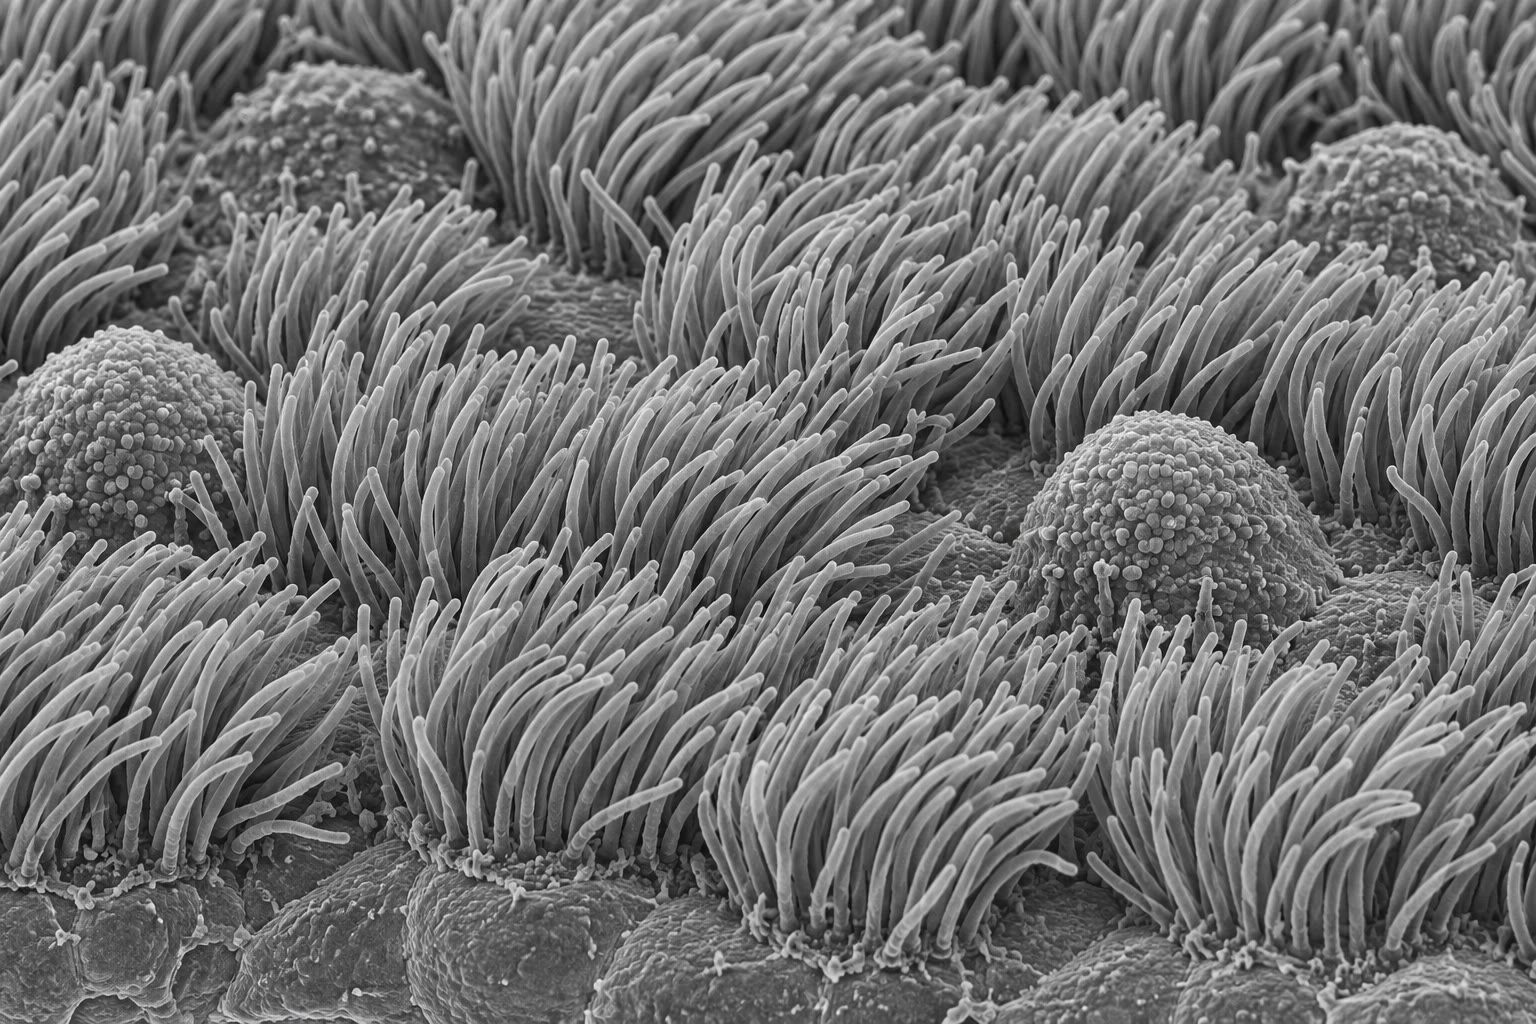
\includegraphics[width=0.54\linewidth]{images/book5/ai/b5-09-cilia-sem.jpg}\hspace{0.03\linewidth}
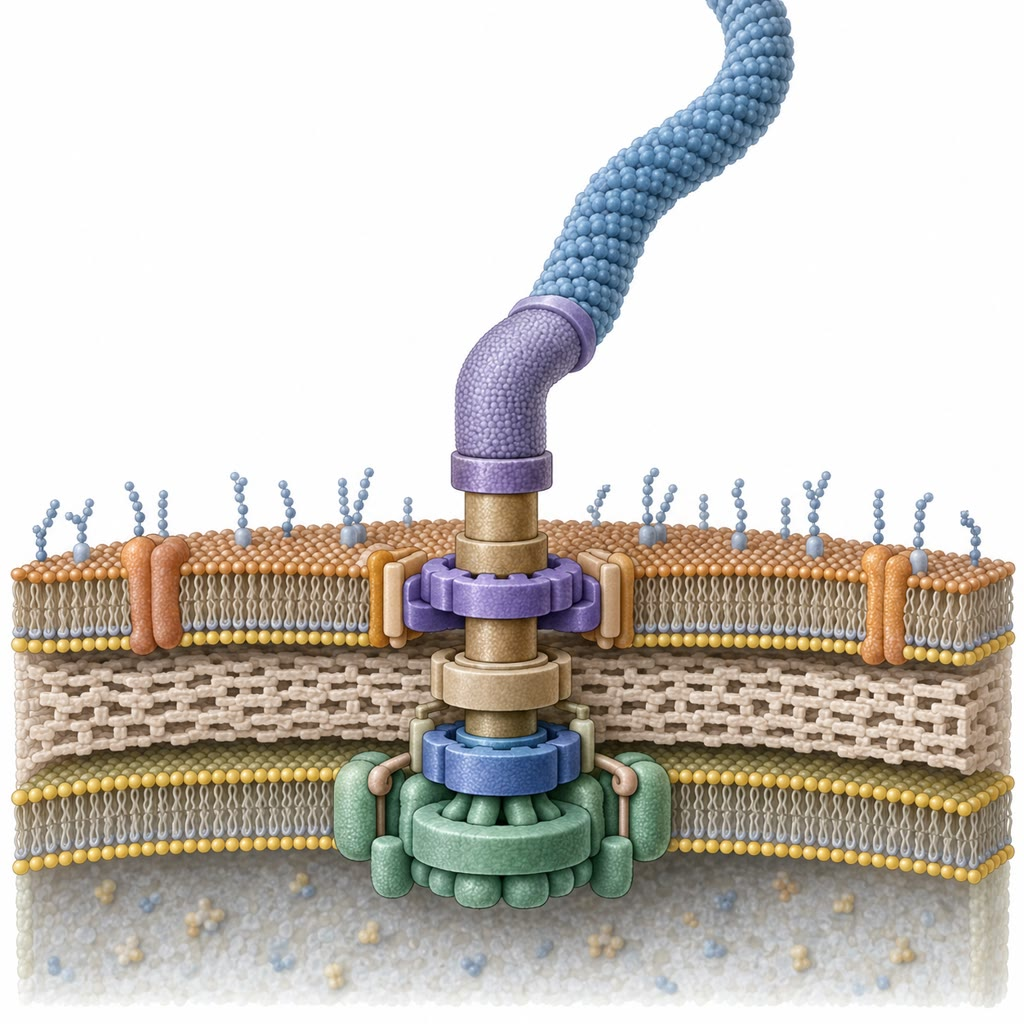
\includegraphics[width=0.36\linewidth]{images/book5/ai/b5-09-flagellar-motor.jpg}

{\small À gauche~: l'épithélium cilié de la trachée au microscope
électronique à balayage, un gazon de \omterm{def:b3:cytoskeleton-motility:cilia}{cils} parmi des cellules en dôme
qui sécrètent le mucus. À droite~: le \omterm{prop:b3:cytoskeleton-motility:flagellar-motor}{moteur flagellaire} bactérien,
machine rotative faite d'anneaux dans l'enveloppe cellulaire et
entraînée par le flux de protons.}
\end{omfigure}

\begin{proposition}[Le moteur flagellaire bactérien]\label{prop:b3:cytoskeleton-motility:flagellar-motor}
\index{moteur flagellaire}\index{course et culbute}
Le flagelle bactérien n'a rien de commun avec celui des eucaryotes~:
c'est un filament hélicoïdal rigide de flagelline, épais de
\qty{20}{nm} et long de plusieurs micromètres, mis en rotation par un
\emph{moteur rotatif} enchâssé dans l'enveloppe cellulaire --- un rotor
d'environ quarante-cinq protéines entouré d'un anneau d'unités
statoriques, chacune un canal par lequel des protons descendent leur
gradient vers l'intérieur, environ mille protons par tour. Le moteur
tourne jusqu'à \qty{300}{Hz}, inverse son sens en une milliseconde et
développe un couple d'environ \qty{1000}{pN.nm}~; il est bâti d'une
vingtaine de protéines dont les gènes s'allument dans l'ordre où les
pièces sont assemblées, du dedans vers le dehors. Chez \emph{E.~coli},
une rotation antihoraire rassemble les quelques flagelles en une hélice
propulsive et la cellule \emph{court} tout droit~; un passage au sens
horaire disperse le faisceau et la cellule \emph{culbute} vers une
nouvelle direction au hasard. La voie du chimiotactisme ne biaise rien
d'autre que la fréquence des culbutes --- moins nombreuses quand les
conditions s'améliorent --- et cela suffit à remonter un gradient.
\end{proposition}

\begin{remark}[Le cytosquelette est un verbe]\label{rem:b3:cytoskeleton-motility:verb}
Presque rien de ce que décrit ce chapitre n'est une structure au sens
où un os en est une~: le \omterm{def:b3:cytoskeleton-motility:migration}{lamellipode} est une onde de polymérisation, le
fuseau du \cref{ch:b3:cell-cycle-apoptosis} un état stationnaire de
\omterm{def:b3:cytoskeleton-motility:filaments}{microtubules} qui croissent et s'effondrent, le battement du \omterm{def:b3:cytoskeleton-motility:cilia}{cil} un
motif de commutation de moteurs. Le renouvellement n'est pas un coût
que la cellule tolère, mais le mécanisme lui-même, ce qui explique que
chacun de ces systèmes tourne à l'hydrolyse d'un nucléotide et
s'arrête quelques minutes après la disparition de l'ATP, et que les
poisons qui figent les polymères dans l'un ou l'autre état --- taxol ou
colchicine, phalloïdine ou cytochalasine --- soient également mortels.
\end{remark}

\section{Exercices}

\begin{exercise}[$\star$]\label{exo:b3:cytoskeleton-motility:1}
Comparer \omterm{def:b3:cytoskeleton-motility:filaments}{filaments d'actine}, \omterm{def:b3:cytoskeleton-motility:filaments}{microtubules} et \omterm{def:b3:cytoskeleton-motility:filaments}{filaments intermédiaires}
par le diamètre, la sous-unité, la polarité, le nucléotide et le rôle
habituel.
\end{exercise}

\begin{exercise}[$\star$]\label{exo:b3:cytoskeleton-motility:2}
Définir la \omterm{thm:b3:cytoskeleton-motility:treadmilling}{concentration critique}. Pourquoi les deux extrémités d'un
\omterm{def:b3:cytoskeleton-motility:filaments}{filament d'actine} ont-elles des \omterm{thm:b3:cytoskeleton-motility:treadmilling}{concentrations critiques} différentes, et
que se passerait-il si elles étaient égales~?
\end{exercise}

\begin{exercise}[$\star$]\label{exo:b3:cytoskeleton-motility:3}
Nommer un moteur pour chacun~: une vésicule vers la périphérie de la
cellule sur des \omterm{def:b3:cytoskeleton-motility:filaments}{microtubules}~; une vésicule vers le centre~; la
contraction d'une fibre de tension~; la courbure d'un \omterm{def:b3:cytoskeleton-motility:cilia}{cil}. Donner le
sens que prend chacun sur sa voie.
\end{exercise}

\begin{exercise}[$\star$]\label{exo:b3:cytoskeleton-motility:4}
Énumérer les quatre étapes du cycle de reptation et la GTPase de la
famille Rho qui gouverne chacune des trois premières.
\end{exercise}

\begin{exercise}[$\star\star$]\label{exo:b3:cytoskeleton-motility:5}
L'extrémité plus d'un polymère a
$k_{\text{on}} = \qty{5}{\micro M^{-1}.s^{-1}}$,
$k_{\text{off}} = \qty{1}{s^{-1}}$, son extrémité moins $k_{\text{on}} =
\qty{1}{\micro M^{-1}.s^{-1}}$, $k_{\text{off}} = \qty{0.8}{s^{-1}}$.
Trouver les deux \omterm{thm:b3:cytoskeleton-motility:treadmilling}{concentrations critiques}, la concentration
stationnaire et la vitesse de treadmilling en sous-unités par seconde
et, pour des sous-unités de \qty{2.7}{nm}, en nanomètres par seconde.
\end{exercise}

\begin{exercise}[$\star\star$]\label{exo:b3:cytoskeleton-motility:6}
La \omterm{def:b3:cytoskeleton-motility:motors}{kinésine} marche à \qty{800}{nm/s} par pas de \qty{8}{nm}, un ATP
chacun. Combien d'ATP par seconde et par moteur~? L'axone d'un neurone
fait \qty{1}{m}~: combien dure le voyage, et combien d'ATP un moteur y
dépense-t-il~? Comparer au temps de diffusion de la
\cref{prop:b3:cytoskeleton-motility:physics}.
\end{exercise}

\begin{exercise}[$\star\star$]\label{exo:b3:cytoskeleton-motility:7}
La \omterm{def:b3:cytoskeleton-motility:motors}{myosine}~V fait des pas de \qty{36}{nm} par ATP. Quelle est sa \omterm{prop:b3:cytoskeleton-motility:physics}{force
d'arrêt} maximale, et pourquoi est-elle plus faible que celle de la
\omterm{def:b3:cytoskeleton-motility:motors}{kinésine}~? Lequel des deux moteurs convient le mieux à une lourde
charge, et lequel à un déplacement rapide~?
\end{exercise}

\begin{exercise}[$\star\star$]\label{exo:b3:cytoskeleton-motility:8}
Prévoir l'effet, sur une cellule en division et sur une cellule qui
rampe, (a) du taxol, (b) de la colchicine, (c) de la cytochalasine,
(d) d'un inhibiteur de Rac, et expliquer chacun par le mécanisme.
\end{exercise}

\begin{exercise}[$\star\star$]\label{exo:b3:cytoskeleton-motility:9}
Dans une expérience de FRAP sur un \omterm{def:b3:cytoskeleton-motility:migration}{lamellipode}, la fluorescence revient
avec un temps de demi-retour de \qty{20}{s} jusqu'à \qty{90}{\%} de sa
valeur initiale. Quels sont le temps de séjour de l'actine dans le
réseau et la fraction immobile~? Les mouchetures refluent à
\qty{1.5}{\micro m/min} pendant que le bord avance à
\qty{1}{\micro m/min}~: à quelle vitesse l'actine polymérise-t-elle au
bord~?
\end{exercise}

\begin{exercise}[$\star\star\star$]\label{exo:b3:cytoskeleton-motility:10}
Expliquer l'\omterm{def:b3:cytoskeleton-motility:instability}{instabilité dynamique} par la \omterm{def:b3:cytoskeleton-motility:instability}{coiffe GTP}, et montrer
pourquoi une population de \omterm{def:b3:cytoskeleton-motility:filaments}{microtubules} maintenue juste au-dessus de la
\omterm{thm:b3:cytoskeleton-motility:treadmilling}{concentration critique} devient bimodale en longueur au lieu d'être
uniforme. Que gagne la cellule à un comportement qui gaspille du GTP~?
\end{exercise}

\begin{exercise}[$\star\star\star$]\label{exo:b3:cytoskeleton-motility:11}
Une bactérie de \qty{2}{\micro m} nage à \qty{25}{\micro m/s}. Dans
l'eau, à cette échelle, la traînée visqueuse domine et la cellule
s'arrête en moins d'un nanomètre quand le moteur s'arrête. Expliquer
pourquoi un mouvement réciproque (une rame) ne peut pas la propulser
alors qu'une hélice en rotation le peut, et estimer le nombre de
protons que le moteur dépense par seconde à \qty{100}{Hz}.
\end{exercise}

\begin{exercise}[$\star\star\star$]\label{exo:b3:cytoskeleton-motility:12}
Le syndrome de Kartagener --- \omterm{def:b3:cytoskeleton-motility:cilia}{cils} immobiles --- donne une bronchite
chronique, une stérilité masculine et, chez la moitié des patients, un
cœur à droite. Expliquer chacun de ces traits par la biologie de
l'\omterm{def:b3:cytoskeleton-motility:cilia}{axonème}, et dire pourquoi le dernier n'en touche que la moitié.
\end{exercise}

\section{Problème~: un neutrophile en marche}

\begin{problem}[{Problème du week-end --- le budget d'actine d'un
neutrophile dénombré, son treadmilling calculé, le voyage d'une
vésicule le long d'un axone chronométré contre la diffusion, le
rendement d'un moteur mesuré, et la polymérisation du front de
reptation et son coût en ATP établis, pour finir sur la vitesse de
treadmilling, le temps pour traverser un axone et l'ATP qu'un
lamellipode brûle par seconde}]
\label{pb:b3:cytoskeleton-motility:1}
Données~: un neutrophile de \qty{300}{\micro m^3} contient de l'actine à
\qty{200}{\micro M}, à moitié polymérisée~; une sous-unité ajoute
\qty{2.7}{nm} à un filament. Constantes de vitesse de l'actine comme
dans l'\cref{ex:b3:cytoskeleton-motility:actin-numbers}. \omterm{def:b3:cytoskeleton-motility:motors}{Kinésine}~: pas
de \qty{8}{nm}, \qty{800}{nm/s}, \omterm{prop:b3:cytoskeleton-motility:physics}{force d'arrêt} \qty{6}{pN}~; hydrolyse
de l'ATP $\Delta G = \qty{50}{kJ/mol}$~; $k_{B}T = \qty{4.1}{pN.nm}$~;
coefficient de diffusion de la vésicule \qty{1}{\micro m^2/s}~; longueur
de l'axone \qty{1}{m}. Le \omterm{def:b3:cytoskeleton-motility:migration}{lamellipode} est large de \qty{20}{\micro m},
avec $200$ filaments par micromètre de bord, et avance à
\qty{10}{\micro m/min}~; le réseau est désassemblé \qty{3}{\micro m}
derrière le bord.

\medskip
\noindent\textbf{Partie I --- Le budget d'actine.}
\begin{enumerate}
  \item Combien de molécules d'actine la cellule contient-elle, et
        combien sont dans des filaments~?
  \item Quelle longueur totale de filament cela fait-il~? Si le
        filament moyen mesure \qty{0.25}{\micro m}, combien de
        filaments~?
  \item L'actine libre est à \qty{100}{\micro M}, bien au-dessus de la
        \omterm{thm:b3:cytoskeleton-motility:treadmilling}{concentration critique} de l'extrémité barbée. Pourquoi les
        filaments ne croissent-ils pas simplement jusqu'à épuisement du
        monomère~? (Deux protéines.)
  \item Treadmilling in vitro~: calculer $C_{\text{ss}}$ et $J$ à partir
        des constantes de vitesse, et la vitesse de treadmilling en
        nanomètres par seconde et en micromètres par minute.
  \item Dans la cellule la vitesse effective est \qty{1}{\micro m/min}.
        De quel facteur les régulateurs accélèrent-ils le polymère nu~?
  \item Chaque sous-unité en treadmilling coûte un ATP. Si les
        $2\times 10^{5}$ filaments faisaient tous du treadmilling à la
        vitesse cellulaire, combien d'ATP par seconde, et quelle
        fraction cela ferait-il du renouvellement total d'une cellule,
        d'environ $10^{9}$ ATP par seconde~?
\end{enumerate}

\medskip
\noindent\textbf{Partie II --- Une vésicule le long de l'axone.}
\begin{enumerate}[resume]
  \item Combien de temps une vésicule tractée par une \omterm{def:b3:cytoskeleton-motility:motors}{kinésine} met-elle
        à parcourir l'axone, et combien de pas et d'ATP le moteur y
        dépense-t-il~?
  \item Combien de temps mettrait la diffusion sur \qty{1}{m}~? Sur
        \qty{10}{\micro m}, la largeur d'un corps cellulaire~? Que dit
        la comparaison sur les endroits où une cellule peut se fier à
        la diffusion~?
  \item Calculer l'énergie par ATP en joules et en unités de $k_{B}T$.
  \item La force maximale d'un moteur à pas de \qty{8}{nm}, et le
        rendement de la \omterm{def:b3:cytoskeleton-motility:motors}{kinésine} à l'arrêt.
  \item Une vésicule de \qty{100}{nm} de rayon, dans un cytoplasme de
        viscosité \qty{0.01}{Pa.s} (dix fois l'eau), qui se déplace à
        \qty{800}{nm/s}, subit une traînée $F = 6\pi\eta r v$. La
        calculer et la comparer à la \omterm{prop:b3:cytoskeleton-motility:physics}{force d'arrêt}~: combien de moteurs
        faut-il~?
  \item L'axone d'un neurone porte environ $10^{4}$ vésicules à la
        fois. Quelle est la consommation totale d'ATP du transport, par
        seconde, et comment se compare-t-elle au coût de la décharge du
        neurone, d'environ $10^{9}$ ATP par seconde~? Qu'implique cela
        pour un neurone dont les mitochondries défaillent~?
\end{enumerate}

\medskip
\noindent\textbf{Partie III --- Le front.}
\begin{enumerate}[resume]
  \item Convertir la vitesse du bord en nanomètres par seconde, et
        calculer le nombre de sous-unités par seconde que chaque
        filament doit ajouter pour suivre.
  \item Combien de filaments poussent le bord, et combien de
        sous-unités par seconde le bord entier consomme-t-il~?
  \item Chaque sous-unité ajoutée est un ATP hydrolysé puis recyclé.
        ATP par seconde pour la protrusion~; fraction des $10^{9}$ par
        seconde de la cellule.
  \item Le réseau derrière le bord est profond de \qty{3}{\micro m} et
        s'y désassemble. Quelle est la durée de vie d'une sous-unité
        dans le réseau, et combien de sous-unités s'y trouvent à tout
        instant~?
  \item La membrane résiste à la protrusion avec une force d'environ
        \qty{1}{pN} par filament. Calculer le travail fourni par
        sous-unité ajoutée ($F\times \qty{2.7}{nm}$) en $k_{B}T$ et dire
        si le cliquet brownien --- une fluctuation thermique qui ouvre
        un interstice de \qty{2.7}{nm} --- est plausible.
  \item Pourquoi la queue en comète de Listeria n'a-t-elle besoin
        d'aucun moteur, et à quelle vitesse peut-elle pousser si elle
        recrute la même machinerie~?
\end{enumerate}

\medskip
\noindent\textbf{Partie IV --- La direction.}
\begin{enumerate}[resume]
  \item Le neutrophile perçoit un chimioattractant dont la
        concentration croît de \qty{2}{\%} sur sa largeur de
        \qty{10}{\micro m}. Avec \num{50000} récepteurs et un $K_{d}$
        égal à la concentration moyenne, combien de récepteurs de plus
        sont occupés sur la moitié avant que sur la moitié arrière~?
        (Occupation $\theta = C/(C +
        K_{d})$~; prendre la moitié des récepteurs de chaque côté.)
  \item La fluctuation aléatoire du nombre d'occupés d'un côté vaut
        environ la racine carrée de ce nombre. La différence de la
        question 19 est-elle détectable à un instant donné~? En quoi
        une moyenne sur quelques secondes aide-t-elle~?
  \item Quelle GTPase doit être activée à l'avant et laquelle à
        l'arrière pour que la cellule se tourne vers la source~? Que
        ferait une cellule dont Rac serait constitutivement active
        partout~?
  \item La cellule atteint la bactérie en \qty{3}{min} depuis
        \qty{30}{\micro m}. Vérifier la vitesse contre les données.
  \item Une cellule dépourvue d'Arp2/3 se déplace par bourgeonnement
        --- des renflements de membrane poussés par la pression ---
        plutôt qu'autrement. Quelle étape du cycle a été remplacée, et
        que cela dit-il du rôle de l'actine dans les autres étapes~?
  \item Le cycle de reptation entier prend quelques minutes, et pourtant
        la cellule se tourne en quelques secondes quand le gradient se
        déplace. Expliquer, en s'appuyant sur la durée de vie du réseau
        de la question~16.
  \item Résumer~: la vitesse de treadmilling in vitro (question~4), le
        temps qu'une vésicule met à parcourir l'axone (question~7) et
        l'ATP par seconde dépensé pour la protrusion (question~15).
\end{enumerate}
\end{problem}
